\subsection{%
  Теорема Гаусса-Остроградского.%
}

\begin{twocolumns}
  \begin{figure}[H]
  \centering

  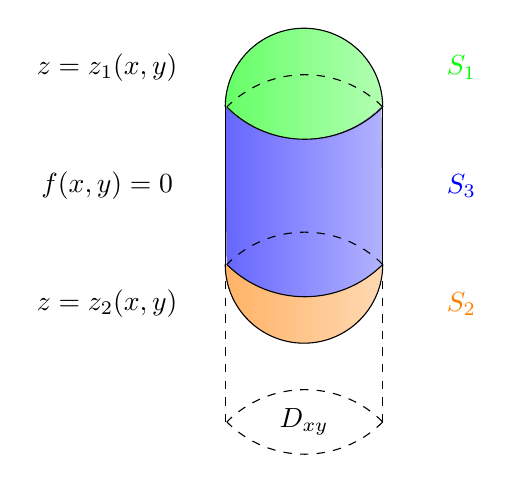
\begin{tikzpicture}
    \fill[left color = green!60, right color = green!30]
      (-1, 2) arc (225 : 315 : 1.4)
      -- (1, 2) arc (0 : 180 : 1)
      -- cycle;

    \fill[left color = blue!60, right color = blue!30]
      (-1, 2) arc (225 : 315 : 1.4)
      -- (1, 0) arc (-45 : -135 : 1.4)
      -- cycle;
  
    \fill[left color = orange!60, right color = orange!30]
      (1, 0) arc (-45 : -135 : 1.4)
      -- (-1, 0) arc (180 : 360 : 1)
      -- cycle;

    \draw (-1, 0) -- (-1, 2);
    \draw (1, 0) -- (1, 2);

    \draw[dashed] (1, 2) arc (45 : 135 : 1.4);
    \draw (1, 2) arc (-45 : -135 : 1.4);
    \draw[dashed] (1, 0) arc (45 : 135 : 1.4);
    \draw (1, 0) arc (-45 : -135 : 1.4);

    \draw (1, 2) arc (0 : 180 : 1);
    \draw (1, 0) arc (0 : -180 : 1);

    \draw[dashed] (1, 0) -- (1, -2);
    \draw[dashed] (-1, 0) -- (-1, -2);

    \draw[dashed] (1, -2) arc (45 : 135 : 1.4);
    \draw[dashed] (1, -2) arc (-45 : -135 : 1.4);
    \draw node at (0, -2) {\(D_{xy}\)};

    \draw node at (2, 2.5) {\textcolor{green}{\(S_{1}\)}};
    \draw node at (2, 1) {\textcolor{blue}{\(S_{3}\)}};
    \draw node at (2, -0.5) {\textcolor{orange}{\(S_{2}\)}};

    \draw node at (-2.5, 2.5) {\(z = z_{1}(x, y)\)};
    \draw node at (-2.5, 1) {\(f(x, y) = 0\)};
    \draw node at (-2.5, -0.5) {\(z = z_{2}(x, y)\)};

  \end{tikzpicture}
\end{figure}

  \columnbreak

  Пусть дано правильное в направлении \(Oz\) замкнутое тело \(T\), образованное
  поверхностями \(S_{1}\), \(S_{2}\) и \(S_{3}\).

  В области, содержащей тело, определена тройка скалярных функций
  \(P(x, y, z)\), \(Q(x, y, z)\), \(R(x, y, z)\), каждая из которых
  дифференцируема и имеет непрерывные частные производные.
\end{twocolumns}
  
\begin{theorem}\label{GO}
  Теорема Гаусса-Остроградского.

  При выполнении условий, описанных выше, справедливо равенство
  
  \begin{align*}
    \iiint_{T} \left(
      \frac{\partial P}{\partial x} +
      \frac{\partial Q}{\partial y} +
      \frac{\partial R}{\partial z}
    \right) \dd x \dd y \dd z
    =
    \oiint_{S_{T}} \left(
      P \cos \alpha +
      Q \cos \beta +
      R \cos \gamma
    \right) \dd \sigma
  \end{align*}
\end{theorem}  
\begin{proof}
  Рассмотрим одну из частей тройного интеграла и перейдем к повторному:

  \begin{align*}
    \iiint_{T} \frac{\partial R}{\partial z} \dd x \dd y \dd z
    = \iint_{D_{xy}} \dd x \dd y \int_{z_{2}(x, y)}^{z_{1}(x, y)}
      \frac{\partial R}{\partial z} \dd z
    = \iint_{D_{xy}} R(x, y, z_{1}(x, y)) \dd x \dd y
      - \iint_{D_{xy}} R(x, y, z_{2}(x, y)) \dd x \dd y
  \end{align*}

  Теперь, используя формулу вычисления \eqref{eq:surf-int-proj-calc} в обратную
  сторону, перейдем к поверхностному интегралу:
  
  \begin{align*}
    \iint_{D_{xy}} R(x, y, z_{1}(x, y)) \dd x \dd y
      - \iint_{D_{xy}} R(x, y, z_{2}(x, y)) \dd x \dd y
    = \iint_{S_{1}^{+}} R(x, y, z) \dd x \dd y
      + \iint_{S_{2}^{-}} R(x, y, z) \dd x \dd y
  \end{align*}

  Заметим, что

  \begin{align*}
    \gamma_{3} = 90 \degree
    \implies \cos \gamma_{3} \dd \sigma = 0 = \dd x \dd y
    \implies \iint_{S_{3}^{+}} R(x, y, z) = 0
  \end{align*}

  поэтому этот интеграл можно добавить к полученному ранее выражению и собрать
  три полученных поверхностных интеграла в один интеграл по поверхности тела:

  \begin{align*}
    \iint_{S_{1}^{+}} R(x, y, z) \dd x \dd y
      + \iint_{S_{2}^{-}} R(x, y, z) \dd x \dd y
      + \iint_{S_{3}^{+}} R(x, y, z) \dd x \dd y
    = \oiint_{S_{T}} R(x, y, z) \dd x \dd y
    = \oiint_{S_{T}} R \cos \gamma \dd \sigma
  \end{align*}

  Таким образом мы получили первое слагаемое в поверхностном интеграле в правой
  части формулы. Аналогично можно показать, что

  \begin{align*}
    \iiint_{T} \frac{\partial P}{\partial x} \dd x \dd y \dd z =
      \oiint_{S_{T}} P \cos \alpha \dd \sigma
    \qquad
    \iiint_{T} \frac{\partial Q}{\partial y} \dd x \dd y \dd z =
      \oiint_{S_{T}} Q \cos \beta \dd \sigma
  \end{align*}
\end{proof}
